\documentclass[11pt]{article}
\usepackage{graphicx} % Required for inserting images
\usepackage{fancyhdr} % Pour personnaliser les en-têtes et les pieds de page
\usepackage{hyperref} % Include the hyperref package
\usepackage{titlesec} % Pour les titres en section
\usepackage{mathptmx} % Times New Roman font
\usepackage{setspace} % Interline spacing
\usepackage{sectsty} % Section styles
\usepackage[backend=biber]{biblatex} %Imports biblatex package
\usepackage{titletoc} % Personalize table of contents
\usepackage{tabularx} % Pour l'environnement tabularx
\usepackage{geometry} % Pour définir les marges
\usepackage{colortbl} % Pour colorer les cases de tableau

% Définition d'une couleur
\definecolor{lightgray}{rgb}{0.8, 0.8, 0.8}

% Définition du fichier de bibliographie
\addbibresource{bibliographie.bib} %Import the bibliography file

% Définition de la commande \subsubsubsection
\titleclass{\subsubsubsection}{straight}[\subsection]
\newcounter{subsubsubsection}[subsubsection]
\renewcommand{\thesubsubsubsection}{\thesubsubsection.\arabic{subsubsubsection}}
\titleformat{\subsubsubsection}{\normalfont\normalsize\bfseries}{\thesubsubsubsection}{1em}{}
\titlespacing*{\subsubsubsection}{0pt}{3.25ex plus 1ex minus .2ex}{1.5ex plus .2ex}

% Définir les marges
\usepackage[top=2.5cm, bottom=2.5cm, left=2.5cm, right=2.5cm]{geometry} % Marges

% Définir le style de la page avec fancyhdr
\pagestyle{fancy}
\fancyhf{} % Effacer les en-têtes et les pieds de page existants

% Définir l'en-tête
\fancyhead[L]{
\includegraphics[height=2cm]{images/univ_lorraine.png}\hspace{0.5cm}
\includegraphics[width=4cm]{images/fst_logo.jpg}} % Image à gauche de l'en-tête

% Supprimer l'alinéa par défaut
\setlength{\parindent}{0pt}

%===================================================================================================%

% Début du rapport
\begin{document}


% Page 1
% Page 1

\begin{center} % Centrer le contenu horizontalement et verticalement
    \vspace*{\fill} % Ajouter de l'espace vertical avant le texte
    \Huge{\textbf{Scanner 3D dense avec couleur}}\\[1cm]
    \Large{Rapport en vue de la validation de l'UE Initiation à la recherche}\\[0.5cm]
    \Large{2023-2024}\\[0.5cm]
    \vspace*{\fill} % Ajouter de l'espace vertical après le texte
\end{center}

% Bloc de texte à gauche
\begin{minipage}[t]{0.75\textwidth}
    \normalsize\textbf{{Etudiants :}}\\
    \normalsize{Sandy GEHIN \\Quentin BELUCHE}
\end{minipage}
% Bloc de texte à droite
\begin{minipage}[t]{0.5\textwidth}
    \normalsize\textbf{{Encadrants :}}\\
    \normalsize{Enseignant-Chercheur\\ Sylvain\\ CONTASSOT-VIVIER \\Doctorant-Chercheur \\Amaury SAINT-JORE}
\end{minipage}

\clearpage

% Page 2
% Page 2
\thispagestyle{empty} % Supprimer l'en-tête et le pied de page
\vspace*{\fill}
\clearpage % Passer à la page suivante

% Page 3
% Page 3
\thispagestyle{empty} % Supprimer l'en-tête et le pied de page
\begin{center}
    \section{\huge\textbf{DÉCHARGES DE RESPONSABILITÉS}}
\end{center}

\normalsize{L’Université de Lorraine n’entend donner ni approbation ni improbation aux opinions émises dans ce rapport, ces opinions doivent être considérées comme propres à leur auteur.}
\clearpage

% Page 4
% Page 4
\thispagestyle{empty} % Supprimer l'en-tête et le pied de page
\begin{center}
    \section{\huge\textbf{{REMERCIEMENTS}}}
\end{center}

\normalsize{
    Merci S. Contassot-Vivier et A. Saint-Jore pour nous avoir donné l'opportunité de découvrir votre travail et de nous avoir donné la chance de pouvoir travailler sur un projet très intéressant.
}
\\ \\
\normalsize{
    Nous tenons à exprimer à S. Contassot-Vivier notre reconnaissance pour votre accompagnement dès le démarrage du projet. Votre expertise et votre guidance nous ont permis de comprendre les complexités de la logique tridimensionnelle et ont été essentielles à chaque étape du processus.
}
\\ \\
\normalsize{
    Nous remercions A. Saint-Jore pour sa confiance et sa générosité en nous prêtant son matériel. Nous sommes reconnaissants de la découverte du monde de la robotique à travers les laboratoires des Mines à Nancy ainsi que du chien robot.
}
\\ \\
\normalsize{
    Un remerciement pour l'équipe des mines du Techlab qui nous a donné sa confiance et l'accès à leurs matériels et locaux.
}

\clearpage

% Page 5
% Page 5
% Personnaliser le formatage du sommaire
\titlecontents{subsubsubsection}[6.3em]{\normalfont\small}{\contentslabel{3.8em}}{}{\titlerule*[1pc]{.}\contentspage}


\thispagestyle{empty} % Supprimer l'en-tête et le pied de page
\begin{center}
    \section{\huge\textbf{{SOMMAIRE}}}  
\end{center}

% Ajoutez la commande suivante pour générer le sommaire automatique
\tableofcontents

\pagestyle{empty} % Supprimer l'en-tête et le pied de page

\clearpage

% Page 6
% Page 5
\thispagestyle{empty} % Supprimer l'en-tête et le pied de page
\begin{center}
    \section{\huge\textbf{{INTRODUCTION}}}  
\end{center}

\subsection{Contexte}
\normalsize{
    \setlength{\parindent}{1cm} % Définir l'alinéa à 1cm à l'intérieur du groupe
    Au sein de l'équipe SIMBIOT, encadrés par S. Contassot-Vivier et A. Saint-Jore, nous allons nous initier dans le domaine de la robotique grâce à un projet intitulé "Développement d'un scanner 3D dense avec couleurs". Notre mission consiste à développer un système de capture générant des nuages denses de points colorés, offrant ainsi un large éventail de possibilités d'application, allant de la cartographie en temps réel à la surveillance environnementale. Cette initiative s'inscrit dans le domaine de l'exploration et de la navigation autonome par robots mobiles, pour par exemple servir un autre projet qui permettra à un chien robot de naviguer dans des grottes, où l'environnement est dense, dangereux, instable et obscure.
}


\\
\subsection{Problèmatique}

\normalsize{
    \setlength{\parindent}{1cm} % Définir l'alinéa à 1cm à l'intérieur du groupe
    L'un des défis majeurs rencontrés dans ce domaine est le développement d'un système de capture capable de générer des nuages denses de points colorés avec une précision et une fidélité optimales. Ces nuages de points constituent une représentation tridimensionnelle détaillée de l'environnement immédiat du robot, fournissant des informations cruciales pour la navigation, la planification de trajectoire et la perception d'objets. Plusieurs questions s'offrent à nous, quelle technologie serait la mieux adaptée à ce projet ? Quelles sont les capacités, le rendu et les différences entre chacune ? Est-ce possible d'avoir un rendu optimal d'un nuage de point colorés?
}

\\
\subsection{Plan}


\normalsize{
    \setlength{\parindent}{1cm} % Définir l'alinéa à 1cm à l'intérieur du groupe
    Pour répondre à cette problématique, notre rapport est structuré autour de plusieurs axes. Tout d'abord, nous procéderons à une étude bibliographique approfondie sur les techniques de scan 3D et de coloriage de points 3D, afin de découvrir ce monde tridimensionnel. Ensuite, nous détaillerons les différentes étapes de nos expérimentations, depuis l'installation et la configuration des équipements de capture jusqu'à la mise en œuvre d'algorithmes de traitement des données et l'évaluation des résultats obtenus. Enfin, nous discuterons des perspectives futures pour notre recherche, en identifiant les défis restants et les pistes d'amélioration envisageables pour faire progresser les technologies de perception pour les robots mobiles autonomes.
}

\clearpage

% Page 7
% Page 7
\pagestyle{empty} % Supprimer l'en-tête et le pied de page
\begin{center}
    \section{\huge\textbf{{DEVELOPPEMENT}}}
\end{center}


\subsection{Etude Bibliographique}
    \subsubsection{Techniques de scan 3D}
        \normalsize{
        \setlength{\parindent}{1cm} % Définir l'alinéa à 1cm à l'intérieur du groupe
            Le choix des Techniques de scan 3D constitue une étape primaire dans le développement de notre système de capture de nuages de points colorés. Cette section vise à explorer les différentes méthodes disponibles, en mettant l'accent sur leur pertinence par rapport à notre projet.
        }

        \subsubsubsection{Scanner 3D à lumière structurée}
            \normalsize{
             \setlength{\parindent}{1cm} % Définir l'alinéa à 1cm à l'intérieur du groupe
                Le scanner 3D à lumière structurée \cite{lumiere_structuree} est une méthode courante de capture de données 3D, qui utilise une lumière projetée sous forme de motif sur la surface de l'objet que l'on souhaite numériser. La déformation de ce motif est ensuite analysée par des capteurs pour calculer les coordonnées tridimensionnelles des points de la surface. Cette technique nous offre une précision accrue, mais peut être limitée par la complexité des formes à numériser et les contraintes environnementales liées à l'utilisation du laser. Cette technique peut être utilisé en temps réel ce qui fait d'elle une candidate potentiel à notre projet.
            }

        \subsubsubsection{Stéréoscopie}
            \normalsize{  
            \setlength{\parindent}{1cm} % Définir l'alinéa à 1cm à l'intérieur du groupe
                La stéréoscopie$^2$ \cite{stereovision} est une approche qui repose sur la capture d'images à partir de plusieurs points de vue pour reconstruire la géométrie tridimensionnelle d'un objet. En comparant les disparités entre les images, il est possible de calculer la profondeur des points de la scène. Cette méthode présente l'avantage de ne pas nécessiter l'utilisation de lasers, mais peut être sensible aux variations d'aclairages et aux occlusions. Nos yeux sont des outils qui utilisent cette technique de perception. Cette technique peut être utilisé en temps réel, elle est souvent utilisée dans la numérisation 3D, la conception assisté par Ordinateur, la réalité augmentée et la robotique, des domaines qui collent parfaitement à notre projet.
            }

        \subsubsubsection{Balayage Laser}
            \normalsize{
                Le balayage laser \cite{balayage_laser} est une technique de scan 3D qui implique l'utilisation d'un laser pour balayer la surface de l'objet à numériser. En mesurant le temps mis par le laser pour rebondir sur la surface et revenir au capteur, il est possible de calculer la distance entre le scanner et chaque point de la surface. Cette méthode est rapide et précise, mais peut être coûteuse et sensible aux matériaux réfléchissants. Cette technique peut être utilisé en temps réel, elle est souvent utilisée dans les domaines, d'ingénierie, d'architecture, d'archéologie et de BTP. Ce qui fait d'elle une redoutable concurrente par son utilisation courante et donc plus approfondie.
            }
            \\ \\
            \normalsize{
                Toutes ces techniques sont des pistes intéressantes à explorer, nous allons donc utiliser, étudier et comparer trois différents outils technologiques qui possèdent chacun leur spécifité, chacun aura une des techniques de scan 3D presentées auparavant.
            }
        
    \subsubsection{Coloriage de points 3D}
        \normalsize{
            L'intégration de la couleur dans les nuages de points 3D est une étape cruciale pour notre projet de développement d'un scanner 3D dense avec couleurs. Cette section se concentre sur les différentes techniques de coloriage des nuages de points tridimensionnels, en mettant en lumière leurs avantages et leurs limitations.
        }
        \\ \\
        \normalsize{
            L'acquisition de couleur dans les nuages de point peut être réalisée de plusieurs manières. La plus courante convient d'utiliser une caméra couleur qui est synchronisée avec le Scanner 3D ce qui permettra d'avoir toutes les informations par rapport aux deux outils, en plus du système NAPS qui nous donne accès à la position en temps réel des outils dans le monde. Toutes ces données nous permettent de faire des calculs grâce à des matrices pour passser du repère 3D au repère de la caméra dans le but de coller chaque points du nuage sur l'image colorée pour ensuite pouvoir récupérer la couleur du pixel correspondante au point puis lui appliquer cette couleur. Suite à cela nous pouvons récupérer le nuage de points coloré en 3D.
        }   
        
    \subsubsection{Mise en place d'emploi du temps}
        \normalsize{
            La gestion et la mise  en place de notre emploi du temps est l'une des étapes les plus importantes pour assurer la progression efficace de notre projet de développement du scanner 3D dense avec couleurs. Cette section détaille l'organisation de nos séances de travails et de nos rencontres avec nos encadrants.
        }
        \\ \\
        \normalsize{
            Nous avons planifié nos séances de travail au Techlab, où nous nous sommes réunis une à deux fois par semaine, soit le matin, soit l'après-midi, en fonction de nos disponibilités et des contraintes de notre emploi du temps respectif. Pendant ces séances, nous avons travaillé sur différents aspects du projet, utilisant tantôt les ordinateurs mis à notre disposition au Techlab, tantôt nos propres ordinateurs, ou encore les équipements spécifiques tels que les jetsons fournies par A. Saint-Jore.
        }
        \\ \\
        \normalsize{
            En plus de nos séances de travail régulières, nous avons eu l'occasion de rencontrer notre encadrant principal, S. Contassot-Vivier, toutes les deux semaines environ. Ces rencontres étaient des moments clés pour discuter de l'avancement du projet, pour nous donner des pistes plus intéressantes à explorer, pour partager nos résultats, nos difficultés, et bénéficer de son expertise. Ces réunions s'effectuaient le plus souvent au Loria.
        }
        \\ \\
        \normalsize{
            Par ailleurs, lors de nos visites au Techlab, nous avons régulièrement croisé A. Saint-Jore, qui nous a apporté un soutien précieux en nous guidant dans l'utilisation des équipements et en répondant à nos questions techniques. Il était aussi présent lors de certaines réunions pour faire le point.
        }
        \\ \\
        \normalsize{
            L'organisation rigoureuse de notre emploi du temps, combinée à nos interactions régulières avec nos encadrants, a favorisé une avancée fluide et efficace de notre projet, nous permettant de relever les défis techniques avec confiance et de progresser vers la réalisation de nos objectifs.
        }


\subsection{Mise en place du montage expérimental}
    \subsubsection{Installation}
        \normalsize{
            Nos encadrants et le Techlab nous ont donc fourni le matériel nécessaires pour réaliser à bien notre projet, cela comprend la caméra Zed2, le Lidar Velodyne Puck Lite etune Jetson. La caméra Zed2 est une caméra composée de deux caméras RGB, celle-ci nous offre une résolution allant jusqu'à 2K, permettant une capture d'images de haute qualité. Elle est dotée de fonctionnalités telles que le contrôle de la caméra, le suivi de position et la détection d'objets. Le Lidar Velodyne Puck Lite utilise des lasers pour une gestion précise de la distance, avec une vitesse de rotation ajustable. Enfin, la Jetson nous offre un ordinateur embarqué qui est prévu d'être implenté dans le robot chien.
        }
        \\ \\
        \normalsize{
            Nous avons entamé la phase d'installation en configurant la caméra Zed2 comme premier dispositif de capture. Étant donné les exigences techniques requises, notamment la nécessité d'une carte graphique Nvidia GTX 1060 au minimum, nous avons dû recourir à l'utilisation de nos propres ordinateurs personnels. L'un de nos deux ordinateurs répondait à ces critères, ce qui nous a conduit à choisir cet équipement pour procéder à l'installation. Cependant, étant donné que cet ordinateur fonctionnait sous le système d'exploitation Windows, cela a entraîné une procédure d'installation différente et plus complexe.
        }
        \\ \\
        \normalsize{
            En ce qui concerne la Kinect v1 et le Velodyne 3D (Lidar), nous avons installé tous les logiciels requis sur nos ordinateurs personnels. Ceux-ci contenant les spécifications adéquates, Windows ne posant aucun problème, nous avons réussi à installer sans problème pour le Lidar le logiciel LidarView \cite{lidarview} et Skanect \cite{skanect} pour la Kinect v1.
        }
        \\ \\
        \normalsize{
            Dans le cadre de l'installation, nous avons téléchargé et configuré plusieurs logiciels et bibliothèques nécessaires, notamment le SDK de la Zed, le SDK d'OpenCV, CUDA, ainsi que des modules Python requis pour le développement ultérieur. Malgré nos efforts, certaines installations, telles que ROS2, ont rencontré des difficultés. Malgré les heures passées à chercher la solution avec l'aide de notre encadrant A. Saint-Jore, nous n'avons pas réussi à installer ROS2. Face à ces problèmes persistants, A. Saint-Jore nous a prêté sa Jetson équipée d'Ubuntu 18 et d'une carte graphique nvidia requise et de 4GB de ram, répondant ainsi aux exigences matérielles nécessaires et offrant une compatibilité adéquate pour nos expériences.
        }
    
    \subsubsection{Configuration des équipements}
        \normalsize{
            Une fois la Jetson mise à notre disposition, nous avons configuré l'environnement de développement en utilisant les ressources du Techlab tels que leurs écrans. Cette étape a impliqué l'installation de ROS2 sur la Jetson, une tâche qui s'est révélée complexe en raison de certaines incompatibilités avec Ubuntu 18. Après avoir identifié la source du problème, nous avons opté pour une version antérieure de ROS2, résolvant ainsi les problèmes de compatibilité et permettant la poursuite de nos expériences.
        }
    
    \subsubsection{Choix de configuration et d'installation}
        \normalsize{
            Suite à ces démarches, nous avons expérimenté avec succès le tutoriel Turtlesim et ROS2 humble \cite{turtle_sim_ros2}, nous familiarisant ainsi avec les principaux concepts de ROS2 tels que les Nodes, les Topics, les Services, et les Paramètres Serveur. Cependant, malgré cette avancée, nous avons rencontré des limitations matérielles avec la Jetson, notamment en termes de mémoire vive insuffisante, ce qui a entravé la génération de nuages de points.
        }
        \\ \\
        \normalsize{
            En effet, un prérequis nous manquait au début mais nous est apparu par la suite, 8GB de ram sont nécessaires au minimum pour permettre à la caméra Zed2 de fonctionner correctement et de générer un nuage de points 3D, ce qui est le double de la jetson.
        }
        \\ \\
        \normalsize{
            En consultation avec nos encadrants, nous avons donc convenu de ne pas poursuivre l'utilisation de ROS2 en raison de ces contraintes matérielles. Néanmoins, cette décision ne nous a pas découragée, car nous avons identifié d'autres possibilités d'utilisation, notamment pour la Zed2, qui peut être utilisé sans ROS2, ce qui nous permet d'avancer dans notre projet avec cet outil.
        }

\subsection{Caméra Zed2}

    \normalsize{
        Sur la caméra Zed2, nous avons effectué un panel de tests, allant d'un simple tutoriel \cite{zed_sdk} de découverte de cet outil jusqu'au détail le concernant. Nous avons testé le control de la caméra, la profondeur, le suivi de position, la détection d'objets, le suivi du corps ainsi que l'enregistrement et la génération d'un nuage de points 3D.
    }

    \subsubsection{Evaluation des résultats}
        \subsubsubsection{Qualité des Images et de la Profondeur}
        \normalsize{
            Lors de nos tests répétés avec la ZED2, nous avons observé une gamme de qualité d'image, allant de médiocre jusqu'à une résolution de 2K, offrant ainsi une variation notable dans la clarté et la netteté des images capturées. Les images de qualité supérieure à 2K ont particulièrement retenu notre attention pour leur excellente qualité visuelle.
        }
        \\ \\
        \normalsize{
            En ce qui concerne la profondeur, nos tests ont révélé des données de profondeur cohérentes et fiables. Les informations de profondeur fournies par la ZED2 semblaient conformes à nos attentes et ont fournies une base solide pour nos expériences ultérieures.
        }
        \\ \\
        \normalsize{
            Sur la base de ces observations, nous avons jugé que la ZED2 présentait des performances acceptables en termes de qualité d'image et de précision de profondeur, ce qui nous a encouragé à poursuivre nos expérimentations, notamment dans la génération de nuages de points.
        }

        \subsubsubsection{Précision du nuage de points}
        \normalsize{
            Pour générer le nuage de points tant attendu, nous avons utilisé un code flexible qui nous permet de modifier plusieurs paramètres pour nous adapter à notre matériel ou à nos besoins spécifiques. Parmi ces paramètres, le DEPTH MODE joue un rôle crucial. Il offre une gamme d'options, allant de NONE à PERFORMANCE, QUALITY, ULTRA, et NEURAL. Le choix du mode de profondeur affecte directement la qualité et la précision du nuage de points généré.
        }
        \\ \\
        \normalsize{
            Le DEPTH MODE détermine la façon dont la ZED2 traite les données de profondeur capturées par ses capteurs. Par exemple, les modes PERFORMANCE et QUALITY peuvent être utilisés pour ajuster la qualité de la profondeur en fonction des exigences de performance du système ou des besoins de qualité d'image. Les modes ULTRA et NEURAL fournissent des niveaux de détail et de précision encore plus élevés, mais peuvent nécessiter plus de ressources matérielles.
        }
        \\ \\
        \normalsize{
            Un autre paramètre crucial est 'camera resolution', qui offre des options telles que VGA, HD720, HD1080 et HD2K. Cette capacité à capturer des images de haute qualité influe directement sur la qualité du nuage de points généré. Des images plus nettes et détaillées se traduiront par un nuage de points plus précis et fidèle à la réalité.
        }
        \\ \\
        \normalsize{
            Suite à la génération des nuages de points, même en qualité maximale, ceux-ci présentaient des imperfections, même avec un nombre élevé de frames. Les murs, le sol et le plafond ne sont pas plats et présentent des irrégularités. Malgré cela, nous avons pu reconnaître en globalité la pièce scannée.
        }
        
        \subsubsubsection{Performance Temporelle}
            \normalsize{
                La performance temporelle de la ZED2 dépend étroitement des deux paramètres principaux mentionnés précédemment, ainsi que du nombre de frames utilisées. En réglant tous les paramètres au minimum avec 80 frames, le temps de traitement est d'environ 2 secondes, en plus du temps nécessaire pour capturer les frames. La reconstruction est généralement satisfaisante, bien que des irrégularités significatives persistent souvent sur les surfaces lisses. Il est important de noter que cette reconstruction est effectuée sans traitement de couleur pour le nuage de points.
            }
            \\ \\
            \normalsize{
                En revanche, en augmentant la qualité des paramètres, le temps de post-traitement$^4$ du nuage de points peut considérablement augmenter. Par exemple, avec une qualité élevée, le temps de post-traitement peut facilement atteindre les 30 secondes, ce qui devient assez long pour des applications nécessitant des résultats rapides.
            }

        \subsubsubsection{Robustesse et fiabilité}
            \normalsize{
                La ZED2 présente une robustesse$^8$ et une fiabilité notables, bien qu'elle puisse rencontrer des défis dans des environnements extrêmes tels que des grottes où la lumière peut être limitée voire inexistante. Son fonctionnement repose sur deux caméras stéréoscopiques qui captent les images et calculent la profondeur en utilisant la disparité entre les images gauche et droite.
            }
            \\ \\
            \normalsize{
                Dans des environnements sombres comme des grottes, la ZED2 peut rencontrer des difficultés en raison du manque de lumière. Bien qu'elle soit équipée de ses propres sources de lumière infrarouge pour aider à la détection de la profondeur dans des conditions de faible luminosité, une source de lumière externe peut être nécessaire pour améliorer la qualité des images et des données de profondeur. La fiabilité de la ZED2 dans de telles conditions dépendra donc de la disponibilité de cette lumière externe et de sa capacité à compenser le manque de luminosité naturelle.
            }
            \\ \\
            \normalsize{
                En termes de robustesse, la ZED2 est conçue pour être utilisée dans une variété de conditions, mais elle peut être sensible aux chocs et aux vibrations excessives, ce qui pourrait affecter sa précision et sa performance. Cette sensibilité est particulièrement pertinente dans le contexte où la caméra est montée sur un chien robot, car elle sera exposée à des vibrations et des mouvements constants pendant son utilisation. Cependant, avec les précautions appropriées et une manipulation soigneuse, la ZED2 peut offrir une fiabilité satisfaisante même dans des environnements difficiles comme des grottes.
            }

\subsection{Kinect v1}

    \subsubsection{Evaluation des résultats}
    
        \subsubsubsection{Qualité des Images et de la Profondeur}
            \normalsize{
                La Kinect datant d'une quinzaine d'années ne permet pas d'obtenir des images de bonne définition, en effet elle ne propose qu'une définition maximum de 480p. Mais si on observe les images obtenues, on peut remarquer que la qualité reste tout de même correct et que le résultat est largement exploitable.
            }
            \\ \\
            \normalsize{
                Pour ce qui est de la profondeur, nous avons obtenu des résultats plutôt corrects où l'on distingue bien les objets selon la distance.
            }
            \\ \\
            \normalsize{
                Selon ces observations, nous pouvons affirmer que la Kinect permet une bonne visualisation du monde qui l'entoure et c'est pourquoi nous avons décidé d'aller plus loin en capturant des nuages de points.
            }
        
        \subsubsubsection{Précision du nuage de points}

            \normalsize{
                En ce qui concerne la capture de nuage de points, nous avons décidé d'utiliser le logiciel Skanect sous Windows. Ce logiciel permet de capturer un nuage de points et de le colorer avec diffrentes qualités. Nous pouvons aussi voir en direct un aperçu 3D coloré de l'image actuelle.
            }
            \\ \\
            \normalsize{
                L'option de reconstruction permet de fusionner chaque nuage de points de chaque frame en un nuage de points complet selon un réglage de qualité allant de LOW à VERY HIGH en passant par MEDIUM et HIGH. Ce paramètre permet d'ajuster la finesse du nuage, c'est à dire la densité$^1$ de points.
            }
            \\ \\
            \normalsize{
                Nous disposons aussi d'une option pour colorier le nuage de points, avec un paramètre de résolution allant de 1 à 20 mm, ainsi que d'autres réglages. Tout cela permet d'obtenir en sortie un nuage de points où chaque point s'est vu attribué une couleur obtenu par l'intermédiaire de la caméra integrée.
            }
            \\ \\
            \normalsize{
                Les nuages de points obtenus par ce logiciel sont assez convaincants, la précision est assez correcte malgré quelques aspérités. On peut noter que la représentation des couleurs est assez fidèle à la réalité mais un peu floue dû à la résolution de la caméra.
            }
        
        \subsubsubsection{Performance Temporelle}
            \normalsize{
                La performance dépend énormement des spécifications de la machine qui exécute Skanect. En effet, la capture des données peut facilement atteindre 60 frames/s, mais à l'étape suivante, c'est-à-dire la fusion, cela peut prendre plus ou moins de temps selon la machine, allant de quelques secondes avec une qualité de fusion basse et un modèle basique jusqu'à plusieurs minutes avec un modèle complexe et une haute qualité pour la fusion.
            }
            \\ \\
            \normalsize{
                En plus de la fusion qui peut prendre un certain temps, en choisissant de colorier le nuage de points après, le logiciel reparcourt une fois de plus la capture pour appliquer la couleur aux points et selon la résolution choisie, le temps de calcul peut s'avérer un peu long tout comme la fusion.
            }

            
        \subsubsubsection{Robustesse et fiabilité}
            \normalsize{
                La Kinect est un capteur plutôt efficace dans les environnements fermés, quelque soit la lumière et même à l'inverse dans un noir le plus total. Cela est du au fait que la Kinect fonctionne avec une lumière structurée emise elle-même par la Kinect. Les espaces restreints ne sont pas un problème pour ce capteur puisque la distance minimale de capture est de quelques dizaines de cm.
            }
            \\ \\
            \normalsize{
                Nous pouvons aussi admirer le fait que la Kinect fonctionne en exterieur malgré qu'avec le soleil qui est une source très importante de lumière peut perturber la lumière structurée émise. Ainsi les nuages de points obtenus peuvent contenir plus d'imprécisions qu'en intérieur. Cela dit la Kinect fonctionne tout de même sans soucis et permet de capturer des données sur plusieurs mètres de distance.
            }


\subsection{Velodyne Puck Lite}
    \subsubsection{Evaluation des résultats}
        \subsubsubsection{Qualité de la Profondeur}
            \normalsize{
                Les tests effectués ont révelés que la gestion de la distance est de très bonne qualité, cela est logique lorsque l'on sait que le lidar fonctionne avec des lasers.
            }
        
        \subsubsubsection{Précision du nuage de points}
            \normalsize{
                Concernant la génération de nuage de points, nous avons utilisé le logiciel LidarView qui permet de récupérer les paquets reseaux envoyés par le lidar sous forme de fichier '.PCAP'. LidarView permet aussi de visualiser en direct le nuage de points actuel capturé par le lidar. Pour finir nous pouvons exporter les points dans un fichier '.ply' par exemple.
            }
            \\ \\
            \normalsize{
                Les nuages de points obtenus par le lidar sont très précis, en effet horizontalement l'angle entre les faisceaux des lasers n'est que de 0,1° ce qui permet une grande densité de points. Verticalement le lidar se révèle moins précis avec un angle de 2° entre chaque faisceau mais si l'on fait bouger le lidar verticalement on peut capturer plus de points et combler les espaces vides verticalement.
            }
            \\ \\
            \normalsize{
                De plus, le Puck Lite permet de capturer environ 600 000 points à la seconde, renvoyant donc des nuages de points très précis et denses.
            }

        \subsubsubsection{Performance Temporelle}
            \normalsize{
                La performance du lidar en terme de temps ne dépend que d'une chose, sa vitesse de rotation. En effet il peut tourner à une vitesse allant de 300 tours/min à 1200 tours/min. Combiné aux 600 000 points capturables par seconde, cela fait donc du lidar une solution très efficace en matière de temps si l'on ne compte pas le post-traitement des nuages de points.
            }
        
        \subsubsubsection{Robustesse et fiabilité}
            \normalsize{
                Le lidar est sûrement l'une des méthodes les plus fiables et robustes pour la capture de points en 3D. Cela se justifie par l'utilisation de lasers, 16 lasers plus précisement. Le calul de distance de chaque faisceau$^5$ est d'une grande précision.
            }
            \\ \\
            \normalsize{
                En plus de ceci, le lidar s'adapte à tous les environnements, que ce soit en intérieur comme en extérieur. Les faisceaux ne sont pas perturbés par la lumière du soleil par exemple. Le seul soucis pourrait être qu'un faisceau qui passe à travers une vitre par exemple ne soit pas réfléchit correctement et conduise donc à une perte de points.
            }
            \\ \\
            \normalsize{
                Enfin, le Puck Lite dispose d'un rayon d'action exemplaire avec une rotation à 360° horizontalement et 30° verticalement. Rajoutons à cela le fait qu'il puisse envoyer des faisceaux à une centaine de mètres de distance et nous avons un moyen fiable et robuste pour capturer des nuages de points.
            }

\subsection{Expérimentations sur des données réelles}
    \subsubsection{Explications}
        \normalsize{
            Suite à nos recherches et à l'évaluation des différentes technologies disponibles, nous avons décidé de nous concentrer sur notre objectif principal : colorier un nuage de points 3D à partir d'un flux d'images. L'un des défis majeurs est de disposer de données de flux d'images ainsi que des informations sur le positionnement de la caméra dans le monde, une tâche complexe sans accès à NAPS. Nous avons décidé avec S. Contassot-Vivier de recourir à des ensembles de données, notamment ceux disponibles sur KITTI \cite{kitti_dataset}. Pour faciliter la manipulation de ces données, nous avons installé Pikitty \cite{kitti_pykitti}, un ensemble de scripts Python spécialement conçu pour le traitement des données KITTI, largement utilisé dans la recherche en vision par ordinateur. Pikitty nous permet d'accéder facilement aux images ainsi qu'aux informations de calibrage de la caméra, des éléments cruciaux pour notre projet. Numpy a aussi été installé pour pouvoir effectuer des calculs matriciels. En exploitant ces données, nous pouvons désormais développer et tester nos algorithmes de coloration avec des données réelles, ce qui nous rapproche fortement de notre but.
        }

    \subsubsection{Réalisations}
        \normalsize{
            À partir de cet ensemble de données complet comprenant les informations de la caméra ainsi que les images correspondantes, nous avons développé un code capable de récupérer des fichiers '.bin' contenant le nuage de points 3D de chaque image. Nous obtenons ainsi une array de points pour chaque image. En parallèle, nous récupérons les données de calibration$^3$ de la caméra ainsi que les données du Velodyne, et nous extrayons les images correspondantes à chaque frame.
        }
        \\ \\
        \normalsize{
            Ensuite, nous utilisons la matrice de projection$^6$ de la caméra, la matrice de réctification et la matrice de transformation du Velodyne à l'image pour effectuer une conversion des points du repère 3D au repère de la caméra. Cette opération implique un calcul matriciel$^7$ expliqué par une revue scientifique \cite{Geiger2013IJRR} en utilisant les produits matriciels de numpy comme suit :
        }
        \\ \\
        \normalsize{
            PointsRepereCamera = MatriceProjectionCamera @ MatriceRectification @ MatriceTransformation @ PointsVelodyne
        }
        \\ \\
        \normalsize{
            Une fois que nous avons réussi à obtenir le nuage de points 3D dans le repère de la caméra, nous sélectionnons les points les plus proches de la caméra, en privilégiant le point le plus proche en cas de superposition de points grâce à un zbuffer. Ensuite, nous colorions chaque point en utilisant la couleur du pixel correspondant dans l'image.
        }
        \\ \\
        \normalsize{
            Enfin, nous affichons les résultats obtenus et récupérons ainsi un nuage de points 3D colorié, résultant de notre processus de traitement et de coloration des données.
        }

    \subsubsection{Analyse}
        \normalsize{
            En analysant notre travail, nous constatons que la récupération du nuage de points 3D colorié a été un succès, ce qui nous permet d'obtenir une représentation tridimensionnelle colorée de notre scène.
        }
        \\ \\
        \normalsize{
            De plus, nous notons que le processus de traitement des données s'est avéré être très rapide, ce qui est un aspect positif en termes d'efficacité et de faisabilité de notre approche. Cela témoigne de l'efficacité de notre code et de notre méthode de traitement des données
        }
        \\ \\
        \normalsize{
            Cependant, malgré ces succès, nous avons fait quelques améliorations dans notre code, puisqu'au début le nuage de points 3D ne faisait pas toute l'image mais était coupé. Grâce à une meilleure gestion des bords nous avons réussi à régler ce problème et à récupérer un nuage de points bien executé. Nous avons aussi dû faire face à un problème avec l'axe Z qui paraissait compressé.
        }


\subsection{Résultats}
    \subsubsection{Comparaisons}
        \normalsize{
            Nous pouvons voir ici les spécifications disponibles pour chacun des 3 appareils (voir Figure \ref{tab:comparison}), lorsque l'on regarde attentivement, on remarque que la ZED est plus performante que la Kinect. Mais lors de nos expérimentations, nous avons des résultats prouvant l'inverse.
        }
        \\ \\
        \normalsize{
            En effet lorsque l'on compare un nuage de points obtenu par la ZED2 (voir Figure \ref{fig:zed2_1}) et un autre par la Kinect (voir Figure \ref{fig:kinect_1)}, on se rend compte que la Kinect produit un résultat bien plus précis, il y a moins d'imperfections contrairement à la ZED2 ou les surface planes ont plus des formes sinusoidales. En revanche si l'on regarde la coloration d'un nuage, la ZED2 (voir Figure \ref{fig:zed2_2}) se trouve être plus performante que la Kinect (voir Figure \ref{fig:kinect_2}) dû à ses caméras de bien meilleure résolution.
        }
        \\ \\
        \normalsize{
           En comparaison avec les deux méthodes précédentes, le lidar (voir Figure \ref{fig:lidar}) se distingue par une précision nettement supérieure dans la génération de nuages de points. En effet, les lignes de points sont parfaitement continues, sans présenter d'aspérités significatives.
        }

    \subsubsection{Conclusions}
        \normalsize{
            En termes de comparaison techniques, sur papier, la caméra zed2 est un technologie qui semble être complète, documentée, avec un accès ouvert aux données grâce à une API dévelopée. Cependant, après expérimentation, on se rend compte que les nuages de points générés par cet outil a premièrement le traitement le plus long de tous les outils, deuxièmement les nuages de points les plus irréguliers et moins complets.
        }
        \\ \\
        \normalsize{
            Contrairement à la Kinect v1 qui nous a surpris nos encadrants et nous, par sa précision. Celle-ci nous donne un nuage de points 3D très bien formé. Son temps de traitement n'est pas le plus rapide mais il faut aussi voir que c'est la première version de cet outil technologique, sortie en 2012, aujourd'hui il y'a de bien meilleures versions, beaucoup plus performant. Cette technologie reste un exploit.
        }
        \\ \\
        \normalsize{
            Pourtant, le lidar est plutôt intéressant, par sa vitesse de traitement, de captures mais aussi par son nuage de points 3D qui nous permet de reconnaître l'environnement, sans grands détails non plus.
        }
        
    
    \subsubsection{Difficultés}

        \normalsize{
            Il est normal de rencontrer diverses difficultés tout au long d'un projet, et le nôtre n'a pas fait exception. Nous avons été confrontés à une série de défis, allant des problèmes d'installation de logiciels à des difficultés matérielles, en passant par des contraintes de puissance de calcul et des incompatibilités matérielles imprévues. Changer de matériel tout en se réadaptant à cette nouvelle technologie et ses exigences propres n'a pas été facile.
        }
        \\ \\
        \normalsize{
            Une des principales difficultés a été le domaine même dans lequel nous nous sommes aventurés, qui s'est avéré être assez complexe et exigeant, surtout sans une expérience préalable significative. Naviguer dans ce territoire inconnu nous a demandé beaucoup d'apprentissage et d'adaptation rapide à de nouveaux concepts et technologies.
        }
        \\ \\
        \normalsize{
            Cependant, nous avons atteint notre but et notre binôme est fier de pouvoir conclure sur ce projet.
        }
\clearpage

% Page 8
% Page 8
\thispagestyle{empty} % Supprimer l'en-tête et le pied de page
\begin{center}
    \section{\huge\textbf{{CONCLUSION}}}
\end{center}

\normalsize{
    En conclusion, notre travail a été guidé par une exploration minutieuse des différentes technologies de capture de données 3D, avec un objectif clair de colorier un nuage de points à partir d'un flux d'images. À travers nos évaluations détaillées de la caméra Zed2, de la Kinect v1 et du Lidar Velodyne Puck Lite, nous avons pu identifier les forces et les limitations de chaque solution. Bien que la Zed2 offre une polyvalence documentée, nous avons constaté que sa performance en matière de traitement des nuages de points était moins satisfaisante que celle de la Kinect v1, qui a été une agréable surprise en termes de précision et de qualité des résultats. Le Lidar Puck Lite, quant à lui, s'est démarqué par sa rapidité de traitement et sa capacité à fournir des nuages de points denses et précis.
}
\\ \\
\normalsize{
    Ce projet nous a permis d'acquérir une compréhension approfondie des technologies de capture 3D et de développer des compétences pratiques dans le traitement et la manipulation de données volumineuses. Nous avons également appris à surmonter des défis techniques et à nous adapter rapidement à de nouveaux concepts et technologies, renforçant ainsi notre capacité à aborder des projets complexes à l'avenir.
}
\\ \\
\normalsize{
    En termes de perspectives futures, notre expérience nous a incités à envisager des développements supplémentaires dans le domaine de la capture et du traitement de données 3D, en particulier en explorant de nouvelles technologies émergentes et en affinant nos méthodes de traitement des nuages de points. Enfin, nous sommes convaincus que les enseignements tirés de cette expérience nous serviront de fondement solide pour aborder de futurs projets avec confiance et compétence.
}

\clearpage

% Page 9
% Page 9
\thispagestyle{empty} % Supprimer l'en-tête et le pied de page
\begin{center}
    \section{\huge\textbf{{ANNEXES}}}
\end{center}

% Sommaire des figures
\phantomsection % Pour que le lien hypertexte pointe au bon endroit
\renewcommand{\listfigurename}{Sommaire des figures} % Nom du sommaire des figures en français
\listoffigures % Sommaire des figures
\addcontentsline{toc}{section}{Sommaire des annexes} % Ajouter au sommaire général

% Sommaire des tables
\phantomsection % Pour que le lien hypertexte pointe au bon endroit
\renewcommand{\listtablename}{Sommaire des tableaux} % Nom du sommaire des tables en français
\listoftables % Sommaire des tables
\clearpage

% Image 1 ZED2 nuage precision
\begin{figure}[h]
    \centering
    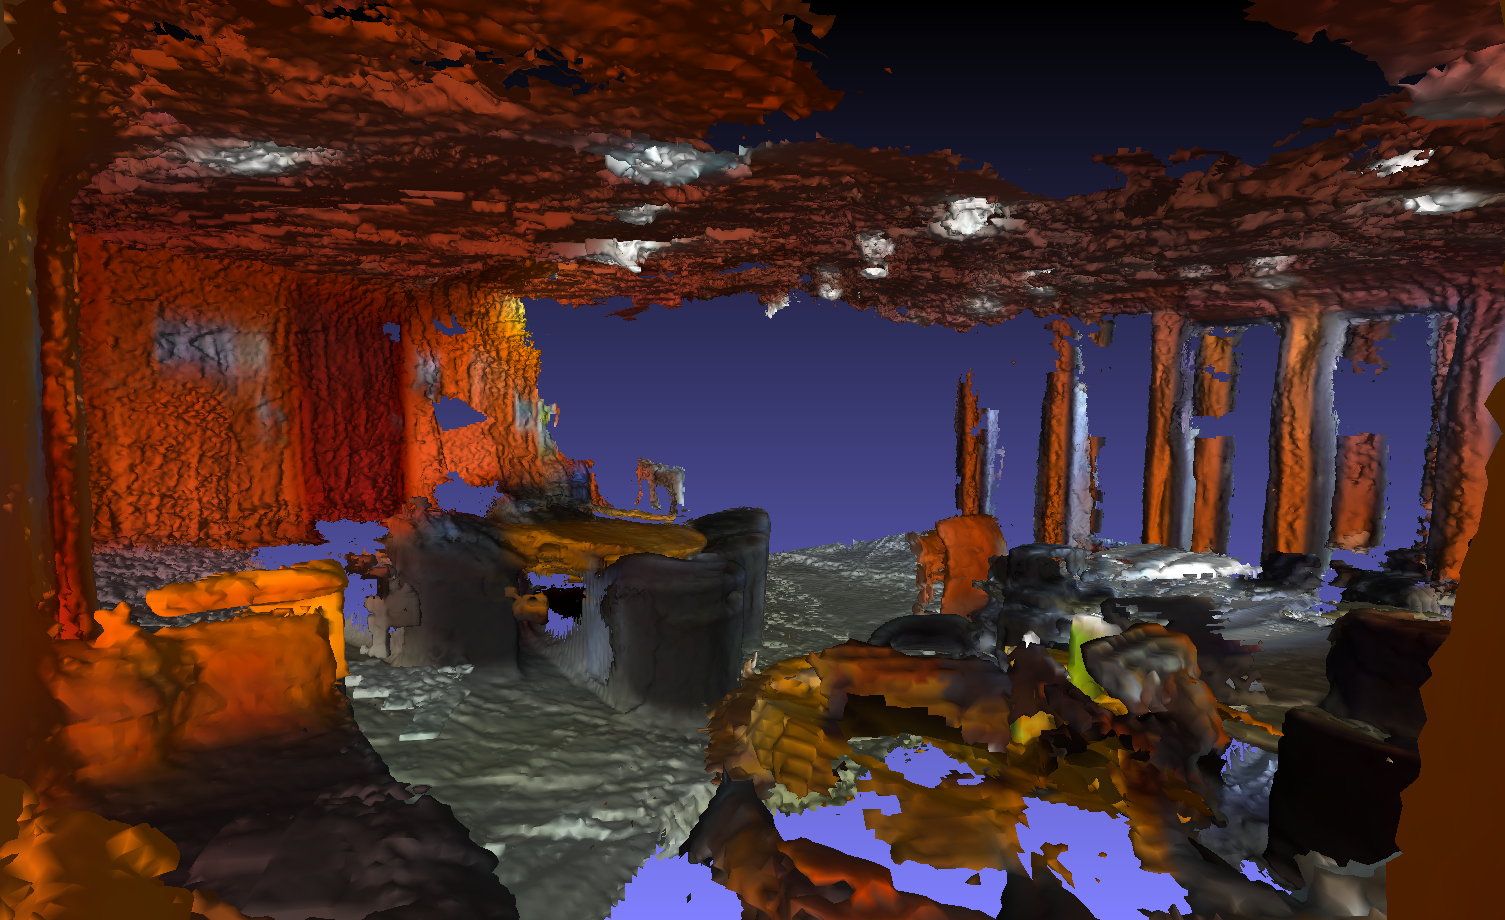
\includegraphics[width=10.5cm]{images/zed2_nuage_colore_2.png}
    \caption{Nuage de points coloré capturé à l'école des Mines de Nancy}
    \label{fig:zed2_1}
\end{figure}

% Image 2 ZED2 nuage coloré
\begin{figure}[h]
    \centering
    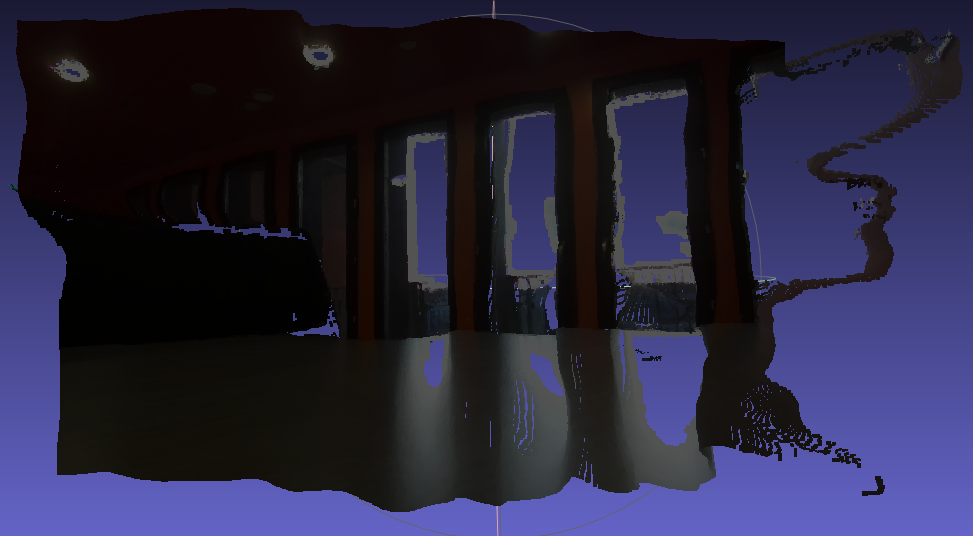
\includegraphics[width=10.5cm]{images/zed2_nuage_colore.png}
    \caption{Nuage de points coloré capturé à l'école des Mines de Nancy}
    \label{fig:zed2_2}
\end{figure}

% Image 1 kinect nuage precision
\begin{figure}[h]
    \centering
    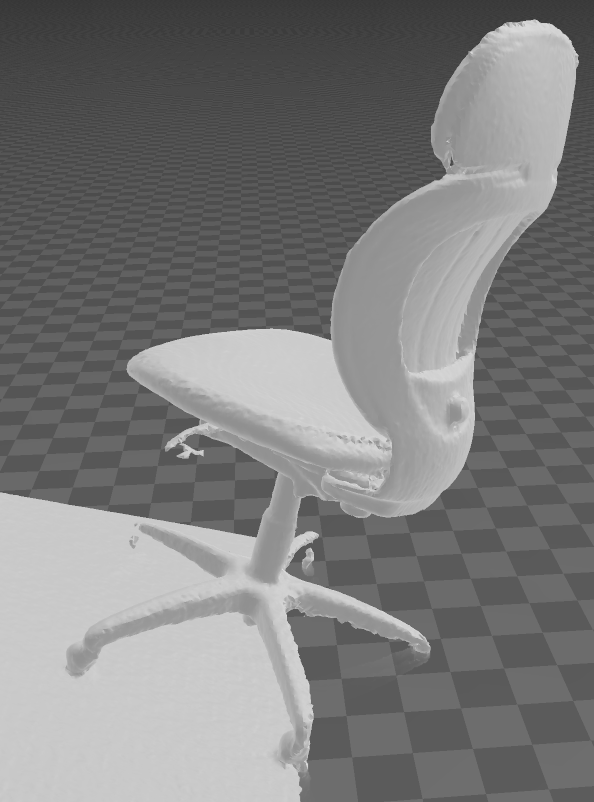
\includegraphics[width=15cm]{images/kinect_sans_couleur.png}
    \caption{Nuage de points brut d'une chaise}
    \label{fig:kinect_1}
\end{figure}


% Image 2 kinect nuage coloré
\begin{figure}[ht]
    \centering
    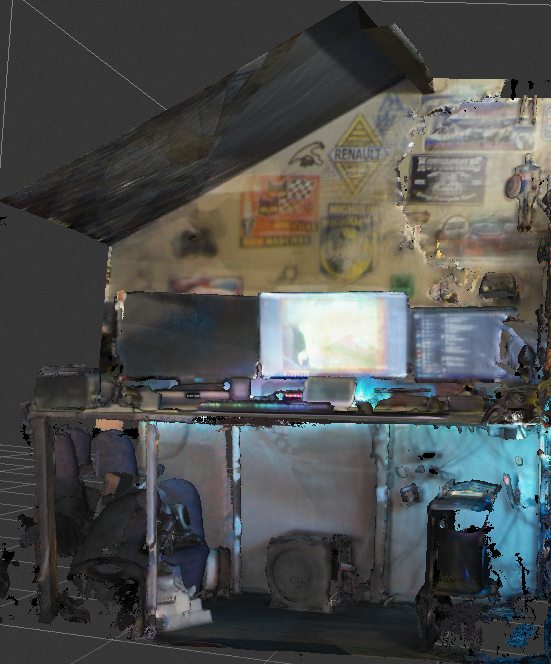
\includegraphics[width=15cm]{images/kinect_avec_couleur.png}
    \caption{Nuage de points coloré d'un bureau}
    \label{fig:kinect_2}
\end{figure}

% Image 1 lidar
\begin{figure}[h]
    \centering
    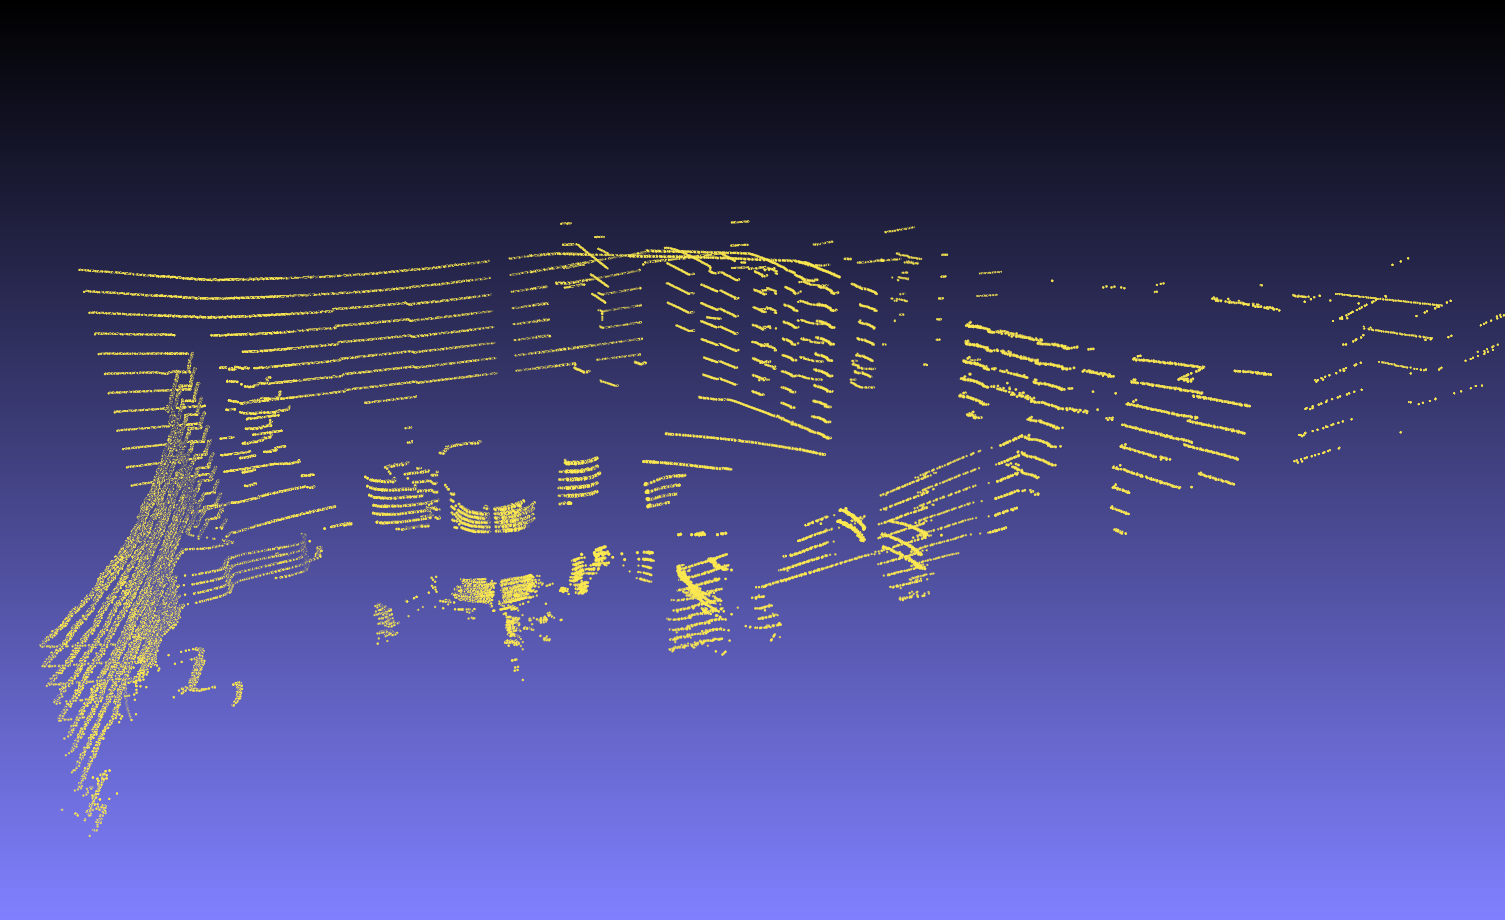
\includegraphics[width=15cm]{images/lidar.png}
    \caption{Nuage de points capturé à l'école des Mines de Nancy}
    \label{fig:lidar}
\end{figure}

\begin{table}[h]
    \centering
    \caption{Comparaison entre ZED 2 / Kinect V1 / Puck Lite}
    \label{tab:comparison}
    \begin{tabularx}{\textwidth}{|>{\hsize=0.6\hsize}X|>{\hsize=0.8\hsize}X|>{\hsize=0.8\hsize}X|>{\hsize=0.8\hsize}X|}
    \hline
    \textbf{Caractéristique} & \textbf{ZED 2} & \textbf{Kinect V1} & \textbf{Puck Lite} \\ \hline
    \textbf{Capture vidéo}    
        & \begin{tabular}[t]{@{}p{1\linewidth}@{}}
            - 2.2K à 15 FPS \\
            - 1080p à 30 FPS \\
            - 720p à 60 FPS \\
            - 376p à 100 FPS
          \end{tabular}
        & \begin{tabular}[t]{@{}p{1\linewidth}@{}}
            - 480p à 30 FPS \\
            - 240p à 30 FPS
          \end{tabular}
        & \cellcolor{lightgray}
        \\ \hline
    \textbf{Vitesse de capture de points} 
        & - 100 Hz 
        & - 30 Hz 
        & \begin{tabular}[t]{@{}p{1\linewidth}@{}} 
          - 300 kHz : en simple \\
          - 600 kHz : en double
          \end{tabular}
        \\ \hline
    \textbf{Vitesse de capture de mouvement} 
        & - 400 Hz 
        & - 30 Hz 
        & \cellcolor{lightgray}
        \\ \hline
    \textbf{Vitesse de capture infrarouge} 
        & \cellcolor{lightgray}
        & - 30 Hz
        & \cellcolor{lightgray}
        \\ \hline 
    \textbf{Densité des nuages} 
        & \cellcolor{lightgray}
        & \cellcolor{lightgray}
        & \begin{tabular}[t]{@{}p{1\linewidth}@{}}
            - $\pm$ 130 pts/mm² à 5 m
          \end{tabular}
        \\ \hline
    \textbf{Précision des points} 
        & $\pm$ 100 mm à 5 m
        & $\pm$ 100 mm à 5 m
        & \begin{tabular}[t]{@{}p{1\linewidth}@{}}
          $\Rightarrow$ $\pm$ 1 mm à 5 m \\
          $\Uparrow$ $\pm$ 3 mm à 5 m
          \end{tabular}
        \\ \hline
    \textbf{Temps de post-traitement}  
        & \begin{tabular}[t]{@{}p{0.8\linewidth}@{}} % 1 => cellule complete 
            De quelques secondes à quelques minutes selon la qualité choisie.
          \end{tabular}
        & \begin{tabular}[t]{@{}p{0.8\linewidth}@{}}
            De quelques secondes à quelques minutes selon la qualité choisie.
          \end{tabular}
        & \begin{tabular}[t]{@{}p{1\linewidth}@{}}
            Quelques secondes.
          \end{tabular}
        \\ \hline
    \textbf{Champ d'action}    
        & \begin{tabular}[t]{@{}p{1\linewidth}@{}}
            $\pm$ 1 m à $\pm$ 20 m
          \end{tabular}
        & \begin{tabular}[t]{@{}p{1\linewidth}@{}}
            $\pm$ 0.8 m à $\pm$ 4 m
          \end{tabular}
        & \begin{tabular}[t]{@{}p{1\linewidth}@{}}
            $\pm$ 0.9 m à $\pm$ 100 m
          \end{tabular}
        \\ \hline
    \textbf{Infos récupérées} 
        & \begin{tabular}[t]{@{}p{0.8\linewidth}@{}}
            - Image RGB x2 \\
            - Nuage de point \\
            - Accéléromètre \\
            - Gyroscope \\
            - Baromètre \\
            - Magnétomètre \\
            - Température
          \end{tabular}
        & \begin{tabular}[t]{@{}p{0.8\linewidth}@{}}
            - Image RGB \\
            - Nuage de point \\
            - Mouvement des objets de son champ de vision \\
            - Microphone
          \end{tabular}
        & \begin{tabular}[t]{@{}p{0.8\linewidth}@{}}
            - Nuage de point \\
            - Mesure de réfléxion \\
            - Angle de rotation \\
            - Horodotage synchronisé \\
            - Position GPS (avec un module en option)
          \end{tabular} 
        \\ \hline
    \textbf{Accès ouvert aux données} 
        & \begin{tabular}[t]{@{}p{0.8\linewidth}@{}} 
          Oui, il existe l'API ZED SDK ainsi que des logiciels.
          \end{tabular}
        & \begin{tabular}[t]{@{}p{0.8\linewidth}@{}} 
          Oui, il existe un kit de développement et un SDK. \\
          Des logiciels tiers sont disponibles comme Skanect ou encore Libfreenect.
          \end{tabular}
        & \begin{tabular}[t]{@{}p{0.8\linewidth}@{}}
            Oui, il existe l'API Paraview ainsi que le logiciel LidarView par exemple.
          \end{tabular}
        \\ \hline
    \end{tabularx}
\end{table}

\clearpage

% Page 10
% Page 10
\thispagestyle{empty} % Supprimer l'en-tête et le pied de page
\begin{center}
    \section{\huge\textbf{{BIBLIOGRAPHIE}}}
\end{center}

% Sites internet
\printbibliography[type=misc,title={Sites internet}]

% Articles
\printbibliography[type=article,title={Articles}]

\clearpage

% Page 11
% Page 11
\thispagestyle{empty} % Supprimer l'en-tête et le pied de page
\begin{center}
    \section{\huge\textbf{{GLOSSAIRE}}}

\end{center}
\textbf{Chaque mot compliqué sera expliqué de manière général et par rapport à notre projet.} \\

\paragraph{$^1$ Densité\label{def:densite}}: La densité se rapporte à la concentration ou au nombre de points dans un nuage de points 3D. Une densité élevée signifierait qu'il y a beaucoup de points dans un espace donné, ce qui peut permettre une représentation plus détaillée d'une surface ou d'un objet.

\paragraph{$^2$ Stéréoscopique\label{def:stereoscopique}}: La stéréoscopie se rapporte à une méthode de capture ou de représentation qui implique deux images (ou plus) prises de points de vue légèrement différents, simulant ainsi la perception de la profondeur

\paragraph{$^3$ Calibration\label{def:calibration}}: La calibration fait référence au processus de réglage et de standardisation des paramètres d'un dispositif de capture pour garantir des mesures précises et cohérentes, dans notre cas ajuster les paramètres du Lidar et de la Zed2.

\paragraph{$^4$ Post-traitement\label{def:post_traitement}}: Le post-traitement se réfère aux opérations effectuées sur les données après leur acquisition initiale. Traitement avant utiliastion

\paragraph{$^5$ Faisceaux laser\label{def:faisceau_laser}}: Les faisceaux laser sont des faisceaux lumineux concentrés et cohérents qui peuvent être utilisés pour mesurer des distances avec une grande précision. Dans le contexte du lidar, les faisceaux laser sont émis par le dispositif pour mesurer la distance aux objets environnants, permettant ainsi la création de nuages de points 3D.

\paragraph{$^6$ Matrice de projection\label{def:matric_proj}}: En vision par ordinateur et en traitement d'image, une matrice de projection est une matrice mathématique utilisée pour transformer des points dans un espace vers un autre espace. Cette transformation est essentielle pour projeter les nuages de points 3D sur une image.

\paragraph{$^7$ Traitement matriciel\label{def:traitement_matriciel}}: Le traitement matriciel fait référence à l'utilisation de techniques mathématiques sur des matrices pour effectuer des opérations telles que la multiplication, l'inversion, la factorisation, etc. Dans notre projet, le traitement matriciel est utilisé pour effectuer des multiplications de matrices.

\paragraph{$^8$ Robustesse\label{def:robustesse}}:  La robustesse se rapporte à la capacité d'un système ou d'un dispositif à maintenir sa performance dans des conditions variables ou difficiles. Dans notre contexte, la robustesse des technologies de capture se réfère à leur capacité à fonctionner de manière fiable dans différents environnements et conditions d'éclairage.  

\clearpage

% Page 12
% Page 12
\thispagestyle{empty} % Supprimer l'en-tête et le pied de page
\begin{center}
    \section{\huge\textbf{{DECLARATION CONTRE LE PLAGIAT}}}
\end{center}

% QUENTIN

\includegraphics[height=1.5cm]{images/univ_lorraine.png}
\begin{center}
    \normalsize\textbf{Déclaration sur l’honneur contre le plagiat}
\end{center}
\normalsize{Je soussigné(e),}\\[0.5cm]
\normalsize{Nom, Prénom : BELUCHE Quentin}\\[0.5cm]
\normalsize{Régulièrement inscrit à l’Université de Lorraine}\\
\normalsize{N° de carte d’étudiant : 32013788}\\
\normalsize{Année universitaire : 2023-2024}\\
\normalsize{Niveau d’études : M1}\\
\normalsize{Parcours : Master Informatique}\\
\normalsize{N° UE : UE 811}\\[0.5cm]
\normalsize{Certifie qu’il s’agit d’un travail original et que toutes les sources utilisées ont été indiquées dans leur totalité. Je certifie, de surcroît, que je n’ai ni recopié ni utilisé des idées ou des formulations tirées d’un ouvrage, article ou mémoire, en version imprimée ou électronique, sans mentionner précisément leur origine et que les citations intégrales sont signalées entre guillemets.}\\[0.5cm]
\normalsize{Conformément à la loi, le non-respect de ces dispositions me rend passible de poursuites    devant la commission disciplinaire et les tribunaux de la République Française.}
\\[1cm]

% Texte en bas à droite
\begin{flushright}
    \normalsize{Fait à  Vandoeuvres-lès-Nancy, le 25/01/2024}\\[1cm]
    \normalsize{Signature :}
    
\includegraphics[height=2cm]{images/signature_quentin.png}
\end{flushright}

% Nouvelle page
\newpage
\thispagestyle{empty} % Supprimer l'en-tête et le pied de page

% SANDY

\includegraphics[height=1.5cm]{images/univ_lorraine.png}
\begin{center}
    \normalsize\textbf{Déclaration sur l’honneur contre le plagiat}
\end{center}
\normalsize{Je soussigné(e),}\\[0.5cm]
\normalsize{Nom, Prénom : GEHIN, Sandy}\\[0.5cm]
\normalsize{Régulièrement inscrit à l’Université de Lorraine}\\
\normalsize{N° de carte d’étudiant : 32013550}\\
\normalsize{Année universitaire : 2023-2024}\\
\normalsize{Niveau d’études : M1}\\
\normalsize{Parcours : Master Informatique}\\
\normalsize{N° UE : UE 811}\\[0.5cm]
\normalsize{Certifie qu’il s’agit d’un travail original et que toutes les sources utilisées ont été indiquées dans leur totalité. Je certifie, de surcroît, que je n’ai ni recopié ni utilisé des idées ou des formulations tirées d’un ouvrage, article ou mémoire, en version imprimée ou électronique, sans mentionner précisément leur origine et que les citations intégrales sont signalées entre guillemets.}\\[0.5cm]
\normalsize{Conformément à la loi, le non-respect de ces dispositions me rend passible de poursuites    devant la commission disciplinaire et les tribunaux de la République Française.}
\\[1cm]

% Texte en bas à droite
\begin{flushright}
    \normalsize{Fait à  Vandoeuvres-lès-Nancy, le 25/01/2024}\\[1cm]
    \normalsize{Signature :}
    
\includegraphics[height=2cm]{images/signature_sandy.png}
\end{flushright}

\clearpage

% Page 13
% Page 4
\thispagestyle{empty} % Supprimer l'en-tête et le pied de page
\vspace*{\fill}
\clearpage

% Page 14
% Page 4
\thispagestyle{empty} % Supprimer l'en-tête et le pied de page
\begin{center}
    \section{\huge\textbf{{RESUME FRANCAIS ET ANGLAIS}}}
\end{center}

\subsection{Francais}
    \normalsize{
        Le projet vise à évaluer différentes technologies de capture 3D en vue de développer un système capable de générer des nuages denses de points colorés. Pour se faire, nous avons suivi une méthodologie comprenant trois étapes principales : la sélection des technologies à évaluer, la réalisation de tests et d'expérimentations, et enfin l'analyse des résultats. Nous avons eu la caméra Zed2, la Kinect v1 et le Lidar Velodyne Puck Lite comme technologies à évaluer en fonction de critères tels que la précision, la vitesse de traitement et la qualité des nuages de points générés. Enfin, nous avons analysé les résultats obtenus pour identifier les forces et les faiblesses de chaque technologie et déterminer leur pertinence par rapport à notre objectif de générer des nuages de points colorés denses.  La caméra Zed2 offre une polyvalence documentée mais présente des limitations dans le traitement des nuages de points. La Kinect v1 surprend par sa précision tandis que le Lidar Puck Lite se distingue par sa rapidité de traitement et sa précision. Enfin, nous avons réussi à générer des nuages de points, et à en colorer dans les data set de Kitti grâce aux informations spatiales manquantes qu'ils nous fournissent. Les principales recommandations proposées sont de bien se documenter sur le sujet, sur la technologie et les possibilités de chaque outils mis à notre disposition.
    }

\subsection{Anglais}
    \normalsize{
        The project aims to evaluate different 3D capture technologies in order to develop a system capable of generating dense colored point clouds. To achieve this, we followed a methodology comprising three main steps: selecting the technologies to evaluate, conducting tests and experiments, and finally analyzing the results. We evaluated the Zed2 camera, the Kinect v1, and the Lidar Velodyne Puck Lite based on criteria such as precision, processing speed, and quality of the generated point clouds. Ultimately, we analyzed the results to identify the strengths and weaknesses of each technology and determine their relevance to our goal of generating dense colored point clouds. The Zed2 camera offers well-documented versatility but has limitations in processing point clouds. The Kinect v1 impresses with its precision, while the Lidar Puck Lite stands out for its processing speed and precision. Finally, we succeeded in generating point clouds and coloring them in the Kitti data set using the spatial information they provide. The main recommendations proposed are to thoroughly research the subject, technology, and capabilities of each tool at our disposal.
    }

\clearpage

% Fin du rapport
\end{document}

%\Huge: Environ 24.88 pt
\huge: Environ 20.74 pt
\LARGE: Environ 17.28 pt
\Large: Environ 14.4 pt
\large: Environ 12 pt
\normalsize: Dépend de la classe de document, souvent 10 pt dans les documents de base
\small: Environ 9 pt
\footnotesize: Environ 8 pt
\scriptsize: Environ 7 pt
\tiny: Environ 5 pt%